\chapter{Development}

The result of this research was the development of |miq|, a package manager and
build system for Linux.

miq is a single-file executable that handles the full lifecycle of the build
process of the packages it manages. This stages include:

\begin{enumerate}
    \item Evaluating the expressions that describe packages
    \item Calculating the dependency graph
    \item Fetching the necessary source code
    \item Performing the described build process
    \item Handling the storage and tracking of the installed packages
\end{enumerate}

Therefore, the following sections will all the components that make up miq, and
their interactions.

\section{High level overview}

The development of miq aimed for a modular design, such that
each component didn't have much coupling with the others.
This allows for easy refactoring of parts of the source
code, while leaving the rest of the system untouched. As
such the components of miq can be layed out in figure
\ref{fig:miq-components} .

\begin{figure}[hbtp]
    \centerfloat
    % 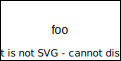
\includegraphics{assets/overview.png}
    \includesvg[width = 450pt]{assets/overview.svg}
    \caption{Overview of the subsystems of miq}
    \label{fig:miq-components}
\end{figure}

Miq is presented as a pipeline of stages, where each
subsystem transform the input data to achieve a desired
state. This design is inspired by other package managers,
which present a similar structure of stages. The main
difference, is that miq works on static package definitions
layed out in a file, which describe the desired state of the
system. In contrast to other package managers, like |apt|,
where the final state of the system is a succession of
commands executed in the shell.

On of the main differences of miq to other package managers,
is how the files are layed out in the filesystem. This is
because each package is given a unique identifier, which in
turns is used for the directory where the package will be
located. This identifier is also unique between different
versions of the same package. And not only that, but it also
encodes the recipe used to build the package itself, and all
of its parents.

To accomplish the tagging of each package with an unique
identifier, a flow of data from package input to package is
visualized on figure \ref{fig:hash}. From a |PackageInput|,
a unique hash is generated, that is the result from hashing
all the fields of the struct. Finally, the hash (an unsigned
32-bit integer) is encoded into text, to form the name of
the package. For this application, the algorithm used is the
\textit{Fowler-Noll-Vo} hash function, which is implemented
in the |fnv| create \cite{FnvRust} . This hash function is
not cryptographically secure, but this was not one of the
design requirements of miq (and can be swapped out for any
other hashing algorithm as needed, as long as it conforms to
the |Hash| trait in Rust).



\begin{minted}{rust}
#[derive(Hash)]
struct PackageInput {
    name: String,
    version: Option<String>,
    script: MetaTextInput,
    deps: Option<Vec<Unit>>,
    env: Option<BTreeMap<String, MetaTextInput>>,
}
\end{minted}

\begin{figure}[hbtp]
    \centerfloat
    \includesvg[width = 0.7\paperwidth ]{assets/hash.svg}
    \caption{Overview of the hashing algorithm}
    \label{fig:hash}
\end{figure}

The implications of this design is that any package gets a
different place on the filesystem, which is derived from
everything that defines the package itself - its build
script and its dependencies, which in turn are also hashed
by the same rules. The advantage of this design, is that
every package has its dependencies perfectly defined,
instead of relying on automatic detection. Let's say that
package |foo| depends of package |bar|. On a conventional
package manager, if |bar| is changed in any form (for
example, updated), then |foo| is usually not modified. But
in essence, now |foo|, if we consider it as a whole, that is
its whole dependency tree, it has changed. This poses a big
issue for the reproducibility of an operating system. Is
|foo| the same if we swapped |bar| for a different version?
Or if we swapped one of |bar|'s dependencies? (Figure
\ref{fig:depswap}) In miq, it is clear that the packages are
no longer the same, as the hashes of its entire dependency
tree has changed, and therefore the name of the output
package. This means that a package "foo" does not really
exist in miq, but rather a package "foo" with a specific hash.

\begin{figure}[hbtp]
    \centerfloat
    \includesvg[width = 200pt]{assets/depswap.svg}
    \caption{Change of dependencies for a package for a conventional package manager}
    \label{fig:depswap}
\end{figure}

% insert depswap-miq.svg
\begin{figure}[hbtp]
    \centerfloat
    \includesvg[width = 200pt]{assets/depswap_miq.svg}
    \caption{Change of dependencies for a package for miq}
    \label{fig:depswap_miq}
\end{figure}

\FloatBarrier
\subsection{Graph-based dependency resolution}

In software deployment, one of the main goals is to have be
able to reproduce a deployment environment as reliably as
possible. This means that any external factors should be
reduced to a minimum, such that the end result is as close
to the expected as possible. The reality of system
deployments is that not all environments are the same, such
that the same deployment can be applied to different systems
with different hardware -- for example, different network
cards, hard drives or even different architectures.

On the software side, the same problem exists. Any
deployment is composed of different parts of software which
interact with each other. To reduce any external factors,
a possible solution is to try to control the entire software
stack -- from the kernel, to the operating system and
libraries and finally to the application to be deployed.
This can be seen in the deployment of an entire \ac{VM}, that
contain the specific OS required for the application. But
this is not always possible, for example in a managed
environment from a cloud provider. Or it may not be desired
for the cost of implementation and maintenance. One of the
most popular solution nowadays is the use of containers
\cite{DockerAcceleratedContainerized2022}. A container is a
collection of files packaged into an \textit{image}, which is
run by a \textit{container runtime}. The runtime is able to
isolate the main process of the container by using special
Linux capabilities, such as \textit{namespaces}
\cite{NamespacesLinuxManualb}. By isolating the ``child''
process from the host, the container is able to bundle its
entire dependency tree without conflicts with the host.

What is proposed in this project is the usage of the hashing
techniques discussed in the previous section to achieve
isolation of the dependency tree of a child process from the
host. Each file which lives in the miq store, has a unique
path according to its hash.

\begin{minted}{bash}
gcc-e3591c92b6d130e5        =>  /miq/store/gcc-e3591c92b6d130e5
bootstrap-5f87f2800c8c639e  =>  /miq/store/bootstrap-5f87f2800c8c639e
\end{minted}

For this reason, a runtime to isolate a process (what is
done with containers) is not needed. Instead, each process
can directly reference the absolute path to the exact
dependency in the store. If package A requires dependency B,
it does not matter if the host \ac{OS} uses also B. If it is
a different version, it will be reflected on its hash -- and
path. If it is exactly the same package B, then the
dependency will be able to be shared across the applications.

\begin{figure}[hbtp]
    \centerfloat
    \includesvg[width=250pt]{assets/depshare.svg}
    \caption{Dependency sharing between applications.}
    \label{fig:dep_share}
\end{figure}

As figure \ref{fig:dep_share} shows, if a there is a
dependency A which is used by two applications, if A is not
the same, the will be no conflict in the file system, as it
will use a different path.

\begin{minted}{bash}
A-1.0.0 => A-1.0.0-1f0d1c2b => /miq/store/A-1.0.0-1f0d1c2b
A-1.0.1 => A-1.0.1-a2b3c4d5 => /miq/store/A-1.0.1-a2b3c4d5
\end{minted}

\FloatBarrier
\subsection{Immutability}

To build reliable system deployments, it is important to reduce the
number of variables that can affect the outcome. From the
software perspective, this means that the system should
either be reliant to changes in the environment, or minimize
the factors from the host that can affect the application.
In Linux, one of the main factors that can affect the
environment are the libraries that are installed on the
system.

On the previous section it was discussed how a different
approach to tagging the packages on the filesystem can be
used to achieve a consistent environment. What this
filesystem layout naturally leads into, is a system where
there is no mutation of the existing packages. On a
classical system, to upgrade a package, the following steps
are taken:

\begin{enumerate}
    \item Download the new update for package |foo|, and unpack it
    \item Replace file |/usr/bin/foo| with the new version
    \item Replace file |/usr/share/foo-bar| with the new version
    \item \ldots
    \item Register the new version in the database
\end{enumerate}

As can be seen, the process of upgrading a package involves
multiple in-place modifications of the existing package.
This operation can be qualified as ``surgical'', as it may
involve many operations which can fail -- and always
eventually fail. This is discussed on section
\ref{sec:atomicity} .

This modification of the global environment poses a problem
to the running processes on the system. Giving names to the
example packages, lets say that |openssl| is updated to a
new version, which fixes some vulnerabilities. The update
process on a classical system would involve replacing
|libcrypto.so| \textbf{in-place} with the new version. But
any running process -- unless it has some internal mechanism
to detect this change -- will be unaware of this change.
Let's say that a package that depends on |openssl| is
|nginx|, which is linked against |libcrypto.so|. Then the
system may be running a vulnerable version of |nginx|, even
if the package was updated. From the perspective of the
package itself, it hasn't changed, yet the underlying
dependency graph as been altered. A solution to this, would
be to track |openssl|'s ``reverse dependencies'', that is,
all packages that depend on it. With this list of reverse
dependencies, one could think that all you need is to
iterate through it, killing every process that depends on
the dependency. But this is not a trivial solution, as there
is no direct connection of running processes to package
versions. For example, the |nginx| package could declare
some systemd service that is part of the package, and then
restart this service in particular. But the system
administrator could as well have written a custom systemd
service, that is not tracked by the package manager. In the
end, the ``safest'' solution, is to just reboot the entire
system after an update has been applied.

\begin{figure}[htb]
    \centerfloat
    \includesvg[width=250pt]{assets/nginx_classic.svg}
    \caption{Tracking reverse dependencies on a classical Linux distribution.}
    \label{fig:nginx_classic}
\end{figure}


So, if in a classical Linux distribution, tracking the files
of the reverse dependencies is not a reliable way to know
when to restart any service that depends on a mutated file,
then the following step could be made: tracking process
uniquely, with some hashing mechanism, such that it can be
known if the reverse dependency (|nginx|) loaded the
vulnerable dependency (|openssl|).


What this naturally leans into, is the solution proposed in this project, of tracking
every package by hashing its entire dependency tree. This
simple change allows to know whether an affected |nginx| is
running against a vulnerable |openssl|, because the
dependency tree is statically known. Because we don't allow
for mutability, every process always runs linked against the
same exact versions of each library. Therefore, if
|libcrypto.so| is updated, some |nginx| processes will still
be linked to the exact path of the old |libcrypto.so| --
|/miq/store/openssl-version-HASH/lib/libcrypto.so|. By
re-evaluating the dependency graph, we can know that the
hash of |nginx| has changed, because it now depends on a
fixed version. Then, from an administrator's perspective,
all you need yo know is to compare the hashes of the old and
new nginx versions, and restart the service such that it
points into the newly-built version.

\begin{figure}[hbtp]
    \centerfloat
    \includesvg[width=250pt]{assets/nginx_miq.svg}
    \caption{Tracking reverse dependencies by hashing the package paths.}
    \label{fig:nginx_miq}
\end{figure}

\FloatBarrier
\subsection{Atomic transactions}
\label{sec:atomicity}

As discussed in the previous section, the usage on mutable
(in-place modifications) systems on Linux, is a serious
source of problems, because of processing tracking a fixed
path of a dependency, that changes under the hood with a
system update. But a different problem that arises from
mutation is the failure of a transaction, that is that a
transaction is ``not atomic''.

Atomicity in software development is a concept usually
associated with memory management. In a multi-threaded
environment, it is important that shared memory is not
written to by two threads at the same time, but
sequentially. For this purpose, the concept of an ``atomic''
operation means that the operation is either not started, or
completed -- there is no state ``in between''
\cite{neelakantamHardwareAtomicityReliable2007} . Using the
similarity with the physical world, an atomic operation is
indivisible.
In the context of package management, we can talk about if a
package manager is atomic, if it can guarantee that a
transaction (for example, updating or installing a package)
is either completed or not, without any intermediate state.

With the analogy of memory for a program, leaving the
filesystem in a intermediate, inconsistent state is not
acceptable for reliable systems. The most basic example is a
package that is being updated, and some error occurs during
the transaction, such that some files have been written, and
some other not, as illustrated in figure
\ref{fig:atomicity}.


\begin{figure}[hbt]
    \centerfloat
    \includesvg[width=200pt]{assets/update_classic.svg}
    \caption{Failure during an update transaction for a
    classical \ac{PM}. Blue: files on the disk after the process.}
    \label{fig:atomicity}
\end{figure}

By having the package manager not rely on the mutation for
upgrades, then the problem of incomplete upgrades is solved
by the root. If mutation is not used, then the way to
upgrade a package is by using a different path on the
filesystem. The upgrade can operate on this different path
completely safely. Any interruption of the process will not
leave the original package in this inconsistent state.
Meanwhile, once the new package is in place, the update
operation is a matter of changing the references of the old
package to the new package.

For the implementation of this concept, in Android the way
to upgrade the system is via A/B updates. The system is partitioned
such that a new update doesn't mutate the existing system,
but rather copied into a different partition. When the
transfer is complete, the user is prompted to reboot the
system, and the bootloader will boot into the new partition.



\subsection{Stages}



\subsection{ELF format}

\subsection{The bootstrapping problem}

\subsection{libc}

\section{Builder}

\section{Graph evaluator}

\section{Lua evaluator}

\section{Other components}

